%%%%%%%%%%%%%%%%%%%%%%%%%%%%%%%%%%%%%%%%%
% Structured General Purpose Assignment
% LaTeX Template
%
% This template has been downloaded from:
% http://www.latextemplates.com
%
% Original author:
% Ted Pavlic (http://www.tedpavlic.com)
%
% Note:
% The \lipsum[#] commands throughout this template generate dummy text
% to fill the template out. These commands should all be removed when 
% writing assignment content.
%
%%%%%%%%%%%%%%%%%%%%%%%%%%%%%%%%%%%%%%%%%

%----------------------------------------------------------------------------------------
%	PACKAGES AND OTHER DOCUMENT CONFIGURATIONS
%----------------------------------------------------------------------------------------
\documentclass{Askarticle}
\usepackage[utf8]{inputenc}
\usepackage{fancyhdr} % Required for custom headers
\usepackage{lastpage} % Required to determine the last page for the footer
\usepackage{extramarks} % Required for headers and footers
\usepackage{graphicx} % Required to insert images
\usepackage{lipsum} % Used for inserting dummy 'Lorem ipsum' text into the template
\usepackage{amsmath}
\usepackage{amsfonts}
\usepackage{listings}
\usepackage{color}
%\usepackage{slashbox}
\usepackage{verbatim}
\usepackage{graphicx}

\usepackage{fancybox}
\usepackage{tikz}

 \usepackage[utf8]{inputenc}
\usepackage[english]{babel}
 
\usepackage{amsthm}
 
\usepackage[colorinlistoftodos]{todonotes}
\usepackage{algorithm}
\usepackage{algpseudocode}

\usepackage{color} %for colored boxes
\usepackage{empheq}

\usepackage{listings} %to include Code

\usepackage{float} %for figs

\usepackage{geometry}
 \geometry{
 a4paper,
 total={210mm,297mm},
 left=20mm,
 right=20mm,
 top=20mm,
 bottom=20mm,
 }

%---------------------------------------------------------------------------------------------
%LISTINGS INITIAL
%---------------------------------------------------------------------------------------------
\definecolor{codegreen}{rgb}{0,0.6,0}
\definecolor{codegray}{rgb}{0.5,0.5,0.5}
\definecolor{codepurple}{rgb}{0.58,0,0.82}
\definecolor{backcolour}{rgb}{0.95,0.95,0.92}
 
\lstdefinestyle{mystyle}{
    backgroundcolor=\color{backcolour},   
    commentstyle=\color{codegreen},
    keywordstyle=\color{magenta},
    numberstyle=\tiny\color{codegray},
    stringstyle=\color{codepurple},
    basicstyle={\ttfamily \footnotesize},
    breakatwhitespace=false,         
    breaklines=true,                 
    captionpos=b,                    
    keepspaces=true,                 
    numbers=left,                    
    numbersep=5pt,                  
    showspaces=false,                
    showstringspaces=false,
    showtabs=false,                  
    tabsize=2
}
 
\lstset{style=mystyle}
%---------------------------------------------------------------------------------------------
% Margins
\topmargin=-0.45in
\evensidemargin=0in
\oddsidemargin=0in
\textwidth=6.5in
\textheight=9.0in
\headsep=0.25in 

\linespread{1.1} % Line spacing

% Set up the header and footer
\pagestyle{fancy}
%\lhead{\hmwkAuthorName} % Top left header
\rhead{\hmwkClass\ : \hmwkTitle} % Top center header
%\chead{\firstxmark} % Top right header
\lfoot{\lastxmark} % Bottom left footer
\cfoot{} % Bottom center footer
\rfoot{Page\ \thepage\ of\ \pageref{LastPage}} % Bottom right footer
\renewcommand\headrulewidth{0.4pt} % Size of the header rule
\renewcommand\footrulewidth{0.4pt} % Size of the footer rule

\setlength\parindent{0pt} % Removes all indentation from paragraphs

%----------------------------------------------------------------------------------------
%	DOCUMENT STRUCTURE COMMANDS
%	Skip this unless you know what you're doing
%----------------------------------------------------------------------------------------

% Header and footer for when a page split occurs within a problem environment
\newcommand{\enterProblemHeader}[1]{
\nobreak\extramarks{#1}{#1 continued on next page\ldots}\nobreak
\nobreak\extramarks{#1 (continued)}{#1 continued on next page\ldots}\nobreak
}

% Header and footer for when a page split occurs between problem environments
\newcommand{\exitProblemHeader}[1]{
\nobreak\extramarks{#1 (continued)}{#1 continued on next page\ldots}\nobreak
\nobreak\extramarks{#1}{}\nobreak
}

\setcounter{secnumdepth}{0} % Removes default section numbers
\newcounter{homeworkProblemCounter} % Creates a counter to keep track of the number of problems

\newcommand{\homeworkProblemName}{}
\newenvironment{homeworkProblem}[1][Problem \arabic{homeworkProblemCounter}]{ % Makes a new environment called homeworkProblem which takes 1 argument (custom name) but the default is "Problem #"
\stepcounter{homeworkProblemCounter} % Increase counter for number of problems
\renewcommand{\homeworkProblemName}{#1} % Assign \homeworkProblemName the name of the problem
\section{\homeworkProblemName} % Make a section in the document with the custom problem count
\enterProblemHeader{\homeworkProblemName} % Header and footer within the environment
}{
\exitProblemHeader{\homeworkProblemName} % Header and footer after the environment
}

\newcommand{\problemAnswer}[1]{ % Defines the problem answer command with the content as the only argument
\noindent\framebox[\columnwidth][c]{\begin{minipage}{0.98\columnwidth}#1\end{minipage}} % Makes the box around the problem answer and puts the content inside
}

\newcommand{\homeworkSectionName}{}
\newenvironment{homeworkSection}[1]{ % New environment for sections within homework problems, takes 1 argument - the name of the section
\renewcommand{\homeworkSectionName}{#1} % Assign \homeworkSectionName to the name of the section from the environment argument
\subsection{\homeworkSectionName} % Make a subsection with the custom name of the subsection
\enterProblemHeader{\homeworkProblemName\ [\homeworkSectionName]} % Header and footer within the environment
}{
\enterProblemHeader{\homeworkProblemName} % Header and footer after the environment
}
   
%----------------------------------------------------------------------------------------
%	NAME AND CLASS SECTION
%----------------------------------------------------------------------------------------
\newcommand\given[1][]{\:#1\vert\:} %define new command
\newcommand{\hmwkTitle}{Homework\ \#3} % Assignment title
\newcommand{\hmwkDueDate}{\today} % Due date
\newcommand{\hmwkClass}{TIM\ 245 - Data Mining} % Course/class
\newcommand{\hmwkClassTime}{4:20pm} % Class/lecture time
\newcommand{\hmwkClassInstructor}{Instructor: Tyler Munger} % Teacher/lecturer
\newcommand{\hmwkAuthorNameB}{Panos Karagiannis}
\newcommand{\hmwkOption}{Homework Heavy Option}
\newcommand{\hmwkIDA}{ID: -}

\newcommand{\Prb}{\mathbb{P}}
\newcommand{\N}{\mathcal{N}}
\newcommand{\R}{\mathbb{R}}
\newcommand{\E}{\mathbb{E}}
\newcommand{\answer}{\noindent\rule{16cm}{0.9pt}
		
		\large{\textbf{\underline{Answer:}}}

		\vspace{0.5cm}}
%----------------------------------------------------------------------------------------
%	TITLE PAGE
%----------------------------------------------------------------------------------------

\title{
\vspace{2in}
\textmd{\textbf{\hmwkClass:\ \hmwkTitle}}\\
\normalsize\vspace{0.1in}\small{Due:\ \textit{\hmwkDueDate}}\\
\vspace{0.1in}\large{\textit{\hmwkClassInstructor}}
\vspace{3in}
}

\author{\begin{tabular}{ l r }
					 \hmwkAuthorNameB \\
					\multicolumn{1}{c}{\hmwkIDA}
				\end{tabular}}
\date{} % Insert date here if you want it to appear below your name

%----------------------------------------------------------------------------------------

\begin{document}

\maketitle

%----------------------------------------------------------------------------------------
%	TABLE OF CONTENTS
%----------------------------------------------------------------------------------------

%\setcounter{tocdepth}{1} % Uncomment this line if you don't want subsections listed in the ToC

\newpage
\tableofcontents
\newpage

\newtheorem{theorem}{Theorem}
\newtheorem{panostheorem}{Theorem}
\newtheorem{claim}[theorem]{Claim}
\newtheorem{definition}[panostheorem]{Definition}

%----------------------------------------------------------------------------------------
%	BLUE BOX
%----------------------------------------------------------------------------------------



\definecolor{myblue}{rgb}{.8, .8, 1}



\newlength\mytemplen
\newsavebox\mytempbox

\makeatletter
\newcommand\mybluebox{%
    \@ifnextchar[%]
       {\@mybluebox}%
       {\@mybluebox[0pt]}}

\def\@mybluebox[#1]{%
    \@ifnextchar[%]
       {\@@mybluebox[#1]}%
       {\@@mybluebox[#1][0pt]}}

\def\@@mybluebox[#1][#2]#3{
    \sbox\mytempbox{#3}%
    \mytemplen\ht\mytempbox
    \advance\mytemplen #1\relax
    \ht\mytempbox\mytemplen
    \mytemplen\dp\mytempbox
    \advance\mytemplen #2\relax
    \dp\mytempbox\mytemplen
    \colorbox{myblue}{\hspace{1em}\usebox{\mytempbox}\hspace{1em}}}

\makeatother

%----------------------------------------------------------------------------------------
%	PROBLEM 1
%----------------------------------------------------------------------------------------

\begin{homeworkProblem}[Problem \arabic{homeworkProblemCounter}: Clustering ]
Using the dataset (\texttt{survey\_dataset.csv})  select one category, e.g. music preferences, to focus on for the \emph{clustering}. Use the selected category and the demographic information to answer the following clustering questions:

\begin{enumerate}
\item Based on the results, which clustering method do you recommend using for the data-set?  Explain why.
\item How many clusters did you find in the dataset? How did you select the method parameters, k or epsilon?
\item Explore the cluster results using Open-Refine or Excel. Pick 2-3 clusters and try to generalize, i.e. create a persona, for the people (instances) in the cluster.
\item  Describe how personas from the clustering results could potentially be used?
\end{enumerate}

\noindent\rule{16cm}{0.9pt}
		
\large{\textbf{\underline{Answer:}}}

This project investigates the clustering results when the \texttt{selected\_category} is \texttt{movies}. Bullet point (1) includes the answer to both questions (1),(2). \\

\begin{enumerate}


\item In order to find the best performing clustering algorithm, given our dataset, we experiment with various clustering models and values of the parameters and report the models for which we obtained the \textbf{highest silhouette score}. We also produce plots by mapping high dimensional data into $2D$ data using \emph{T-SNE}.

\begin{enumerate}
\item The first method that we explore is \emph{K-Means}, which, is a fast and simple approach to clustering which works well for globular clusters. 

\begin{figure}[htp!]
  \begin{center}
  	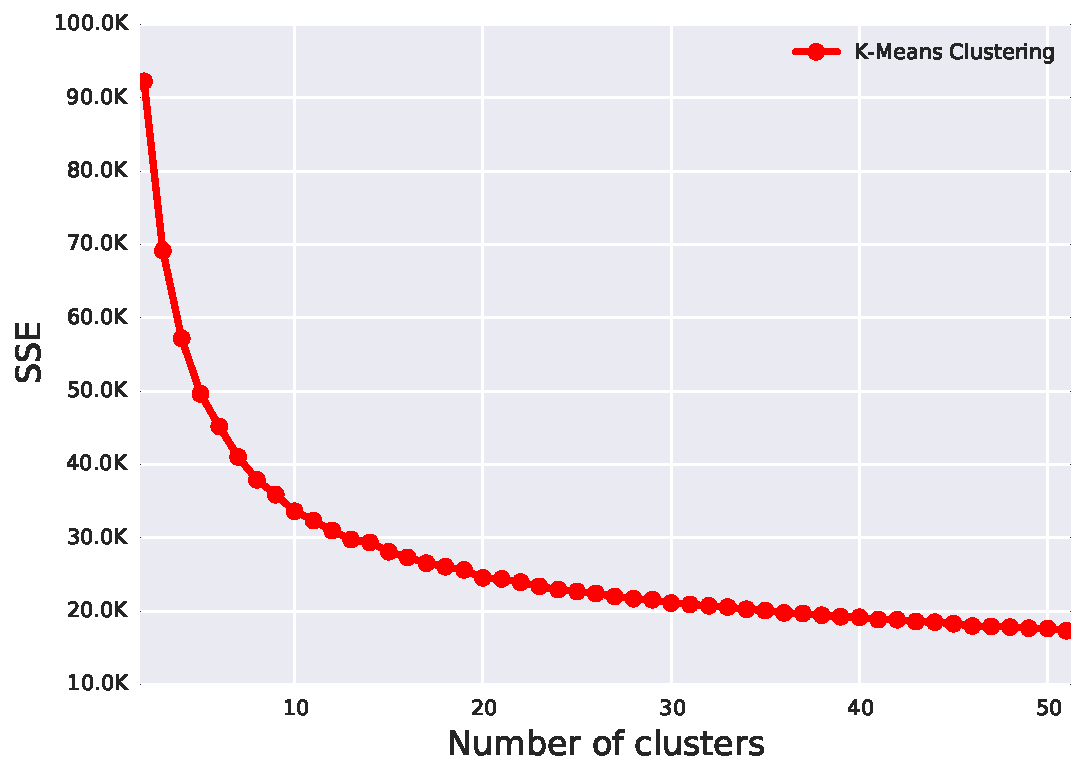
\includegraphics[width=0.6 \textwidth]{../Code/Plots/kmeansse.pdf}
  \end{center}
  \vspace{-.2cm}
  \caption{Sum of squared errors as we vary the number of clusters in the K-Means algorithm.}
  \label{fig:kmeans_elbow}
  \vspace{-.1cm}
\end{figure}

Using the ``elbow method'' we speculate that a useful clustering occurs for a number of clusters between $2$ and $10$ (Fig. \ref{fig:kmeans_elbow}). In order to assess our model we compute the \emph{silhouette} score for all the values of $k=1,2, \dots ,40$ and report the top $4$ models in terms of silhouette score.

\begin{figure}[htp!]
  \begin{center}
  	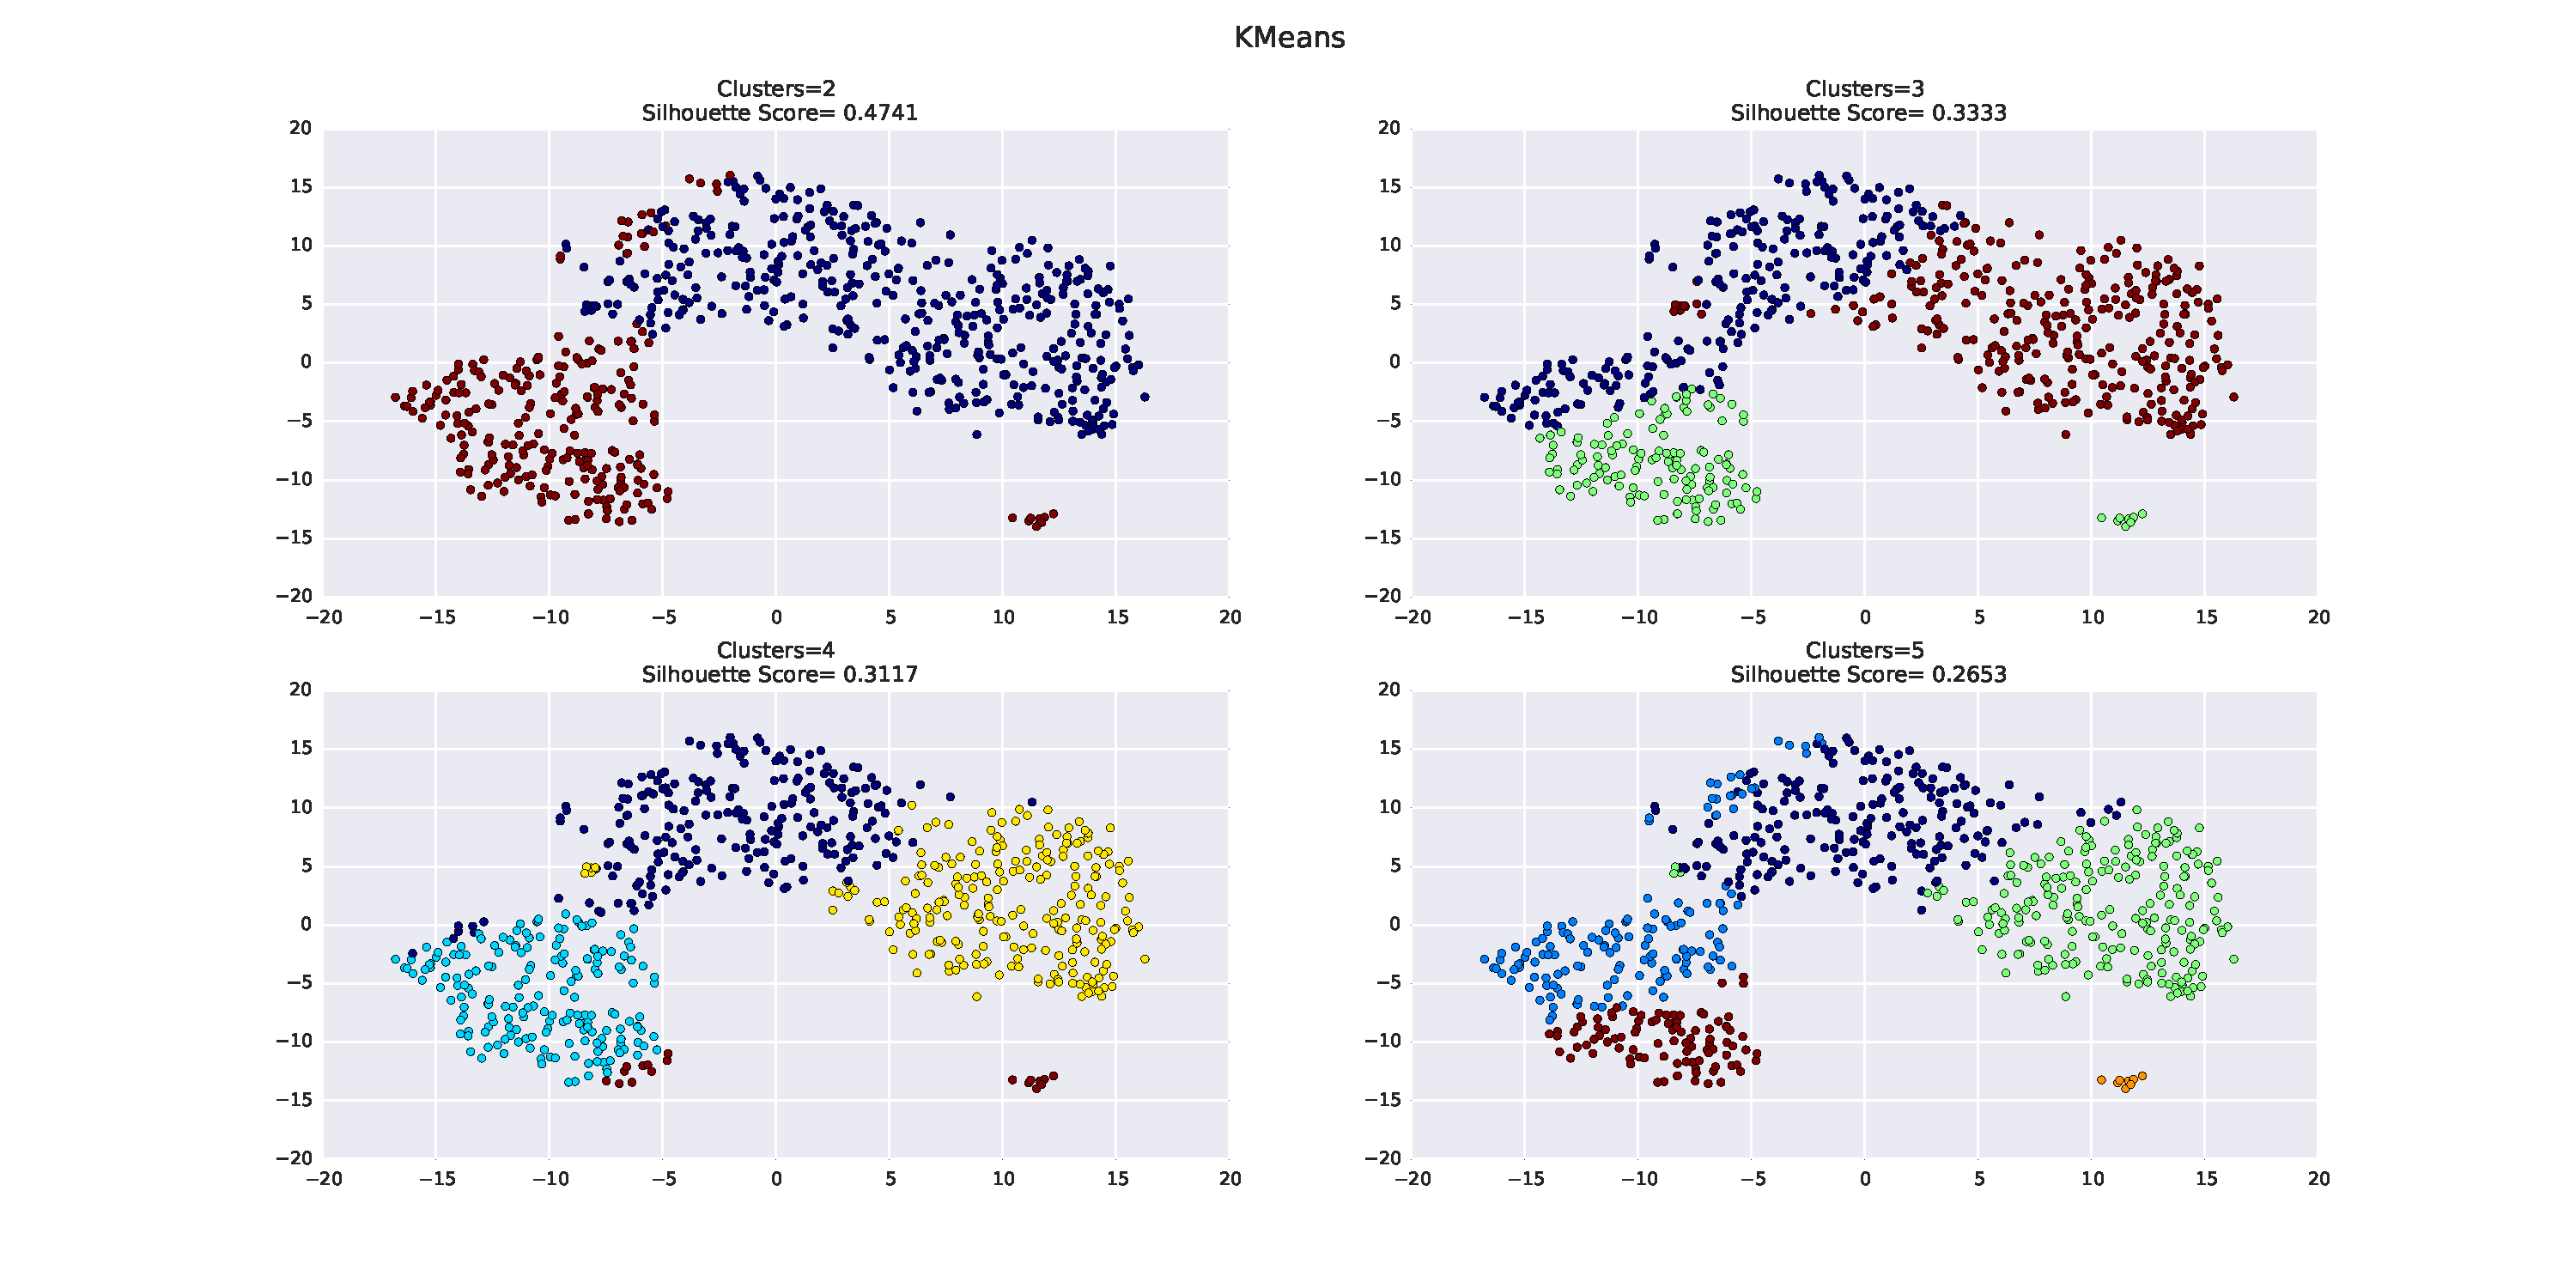
\includegraphics[width=1\textwidth]{../Code/Plots/best_kmeans.pdf}
  \end{center}
  \vspace{-.2cm}
  \caption{Four best K-Means models as we vary $1 \leq k \leq 40$.}
  \label{fig:kmeans_best}
  \vspace{-.1cm}
\end{figure}

As we see from Figure \ref{fig:kmeans_best}, the best silhouette score is achieved for $k=2$ and is equal to $0.4741$. Nevertheless, this silhouette score is still not very close to $1$, therefore, as we see next, K-Means is not the best performing clustering algorithm.


\item The second clustering algorithm that we explore is \emph{Hierarchical Agglomerative Clustering}. In this type of clustering we are given more ``freedom'' than K-Means, in the sense that we can also choose the \emph{linkage} type. More precisely, for Agglomerative Clustering the cost function (linkage) is the distance between clusters. In this project we experiment with all three common linkage methods, namely:
	\begin{itemize}
		\item Single Linkage: The distance between two clusters is the \emph{minimum} distance of their respective points 
		\item Complete Linkage: The distance between two clusters is the \emph{maximum} distance of their respective points 
		\item Average Linkage: The distance between two clusters is the \emph{average} distance of their respective points 
	\end{itemize}

More precisely, for each linkage type we vary the number of clusters $k$ such that $k=1,2 \dots, 40$ \textbf{but only report the four values of $k$ for which we calculated the largest silhouette score.} \\

\begin{figure}[htp!]
  \begin{center}
  	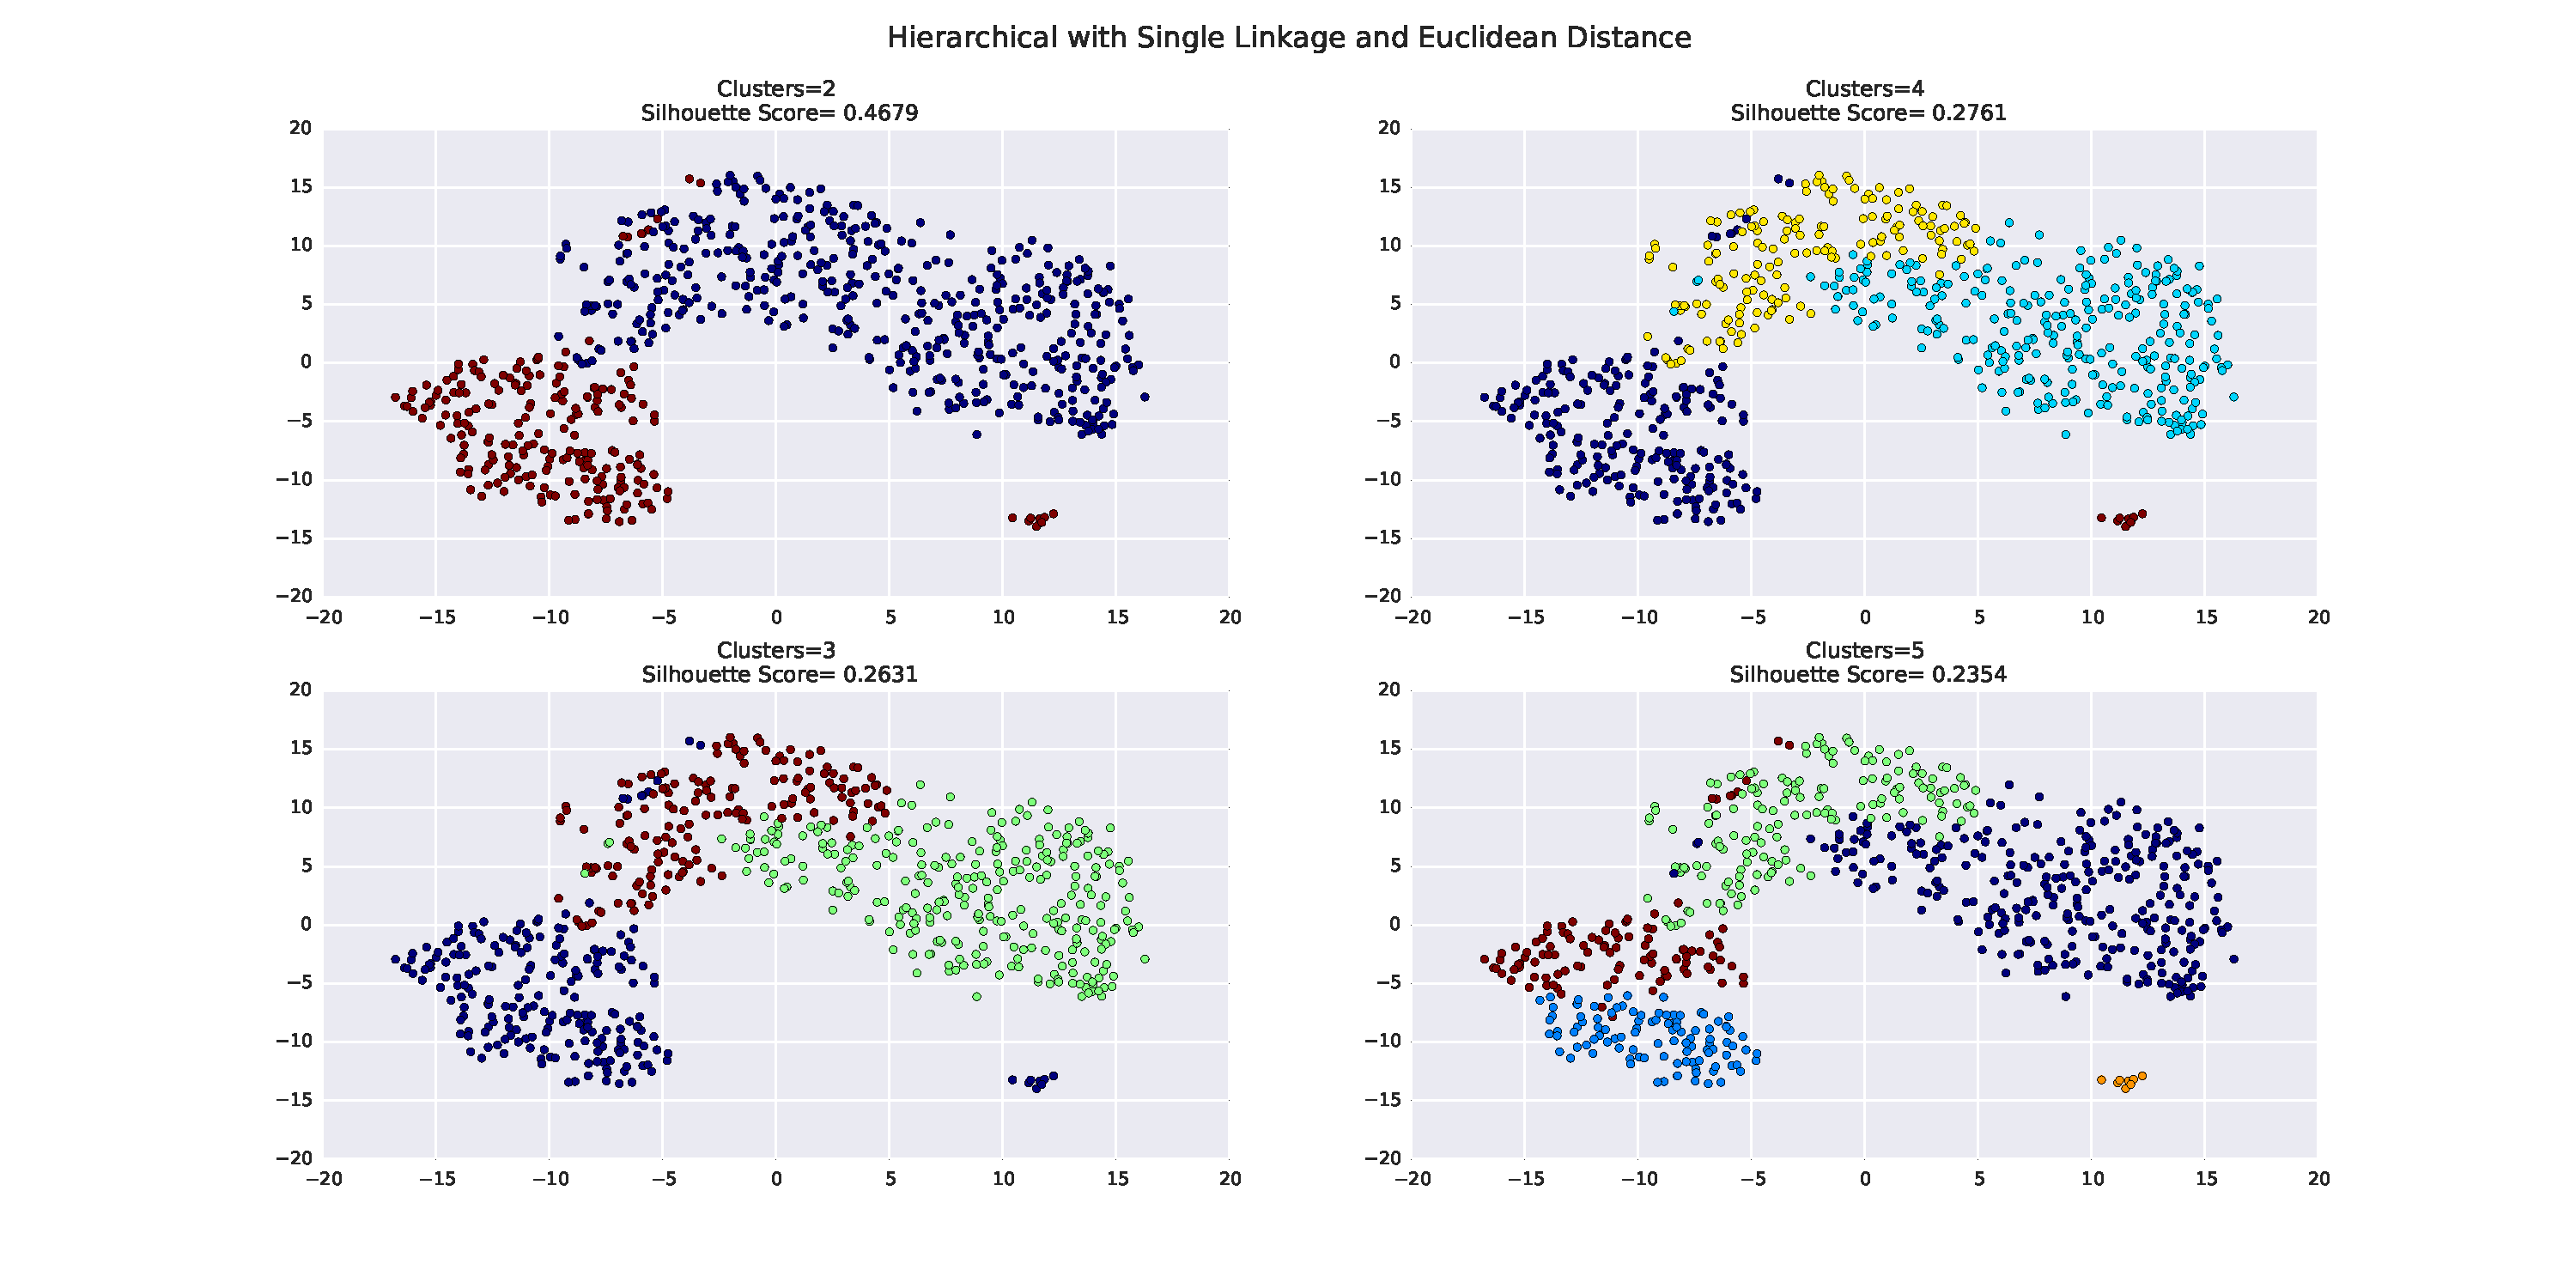
\includegraphics[width=1\textwidth]{../Code/Plots/single_link}
  \end{center}
  \vspace{-.2cm}
  \caption{Four best Single Linkage models as we vary $1 \leq k \leq 40$.}
  \label{fig:single_link}
  \vspace{-.1cm}
\end{figure}

\begin{figure}[htp!]
  \begin{center}
  	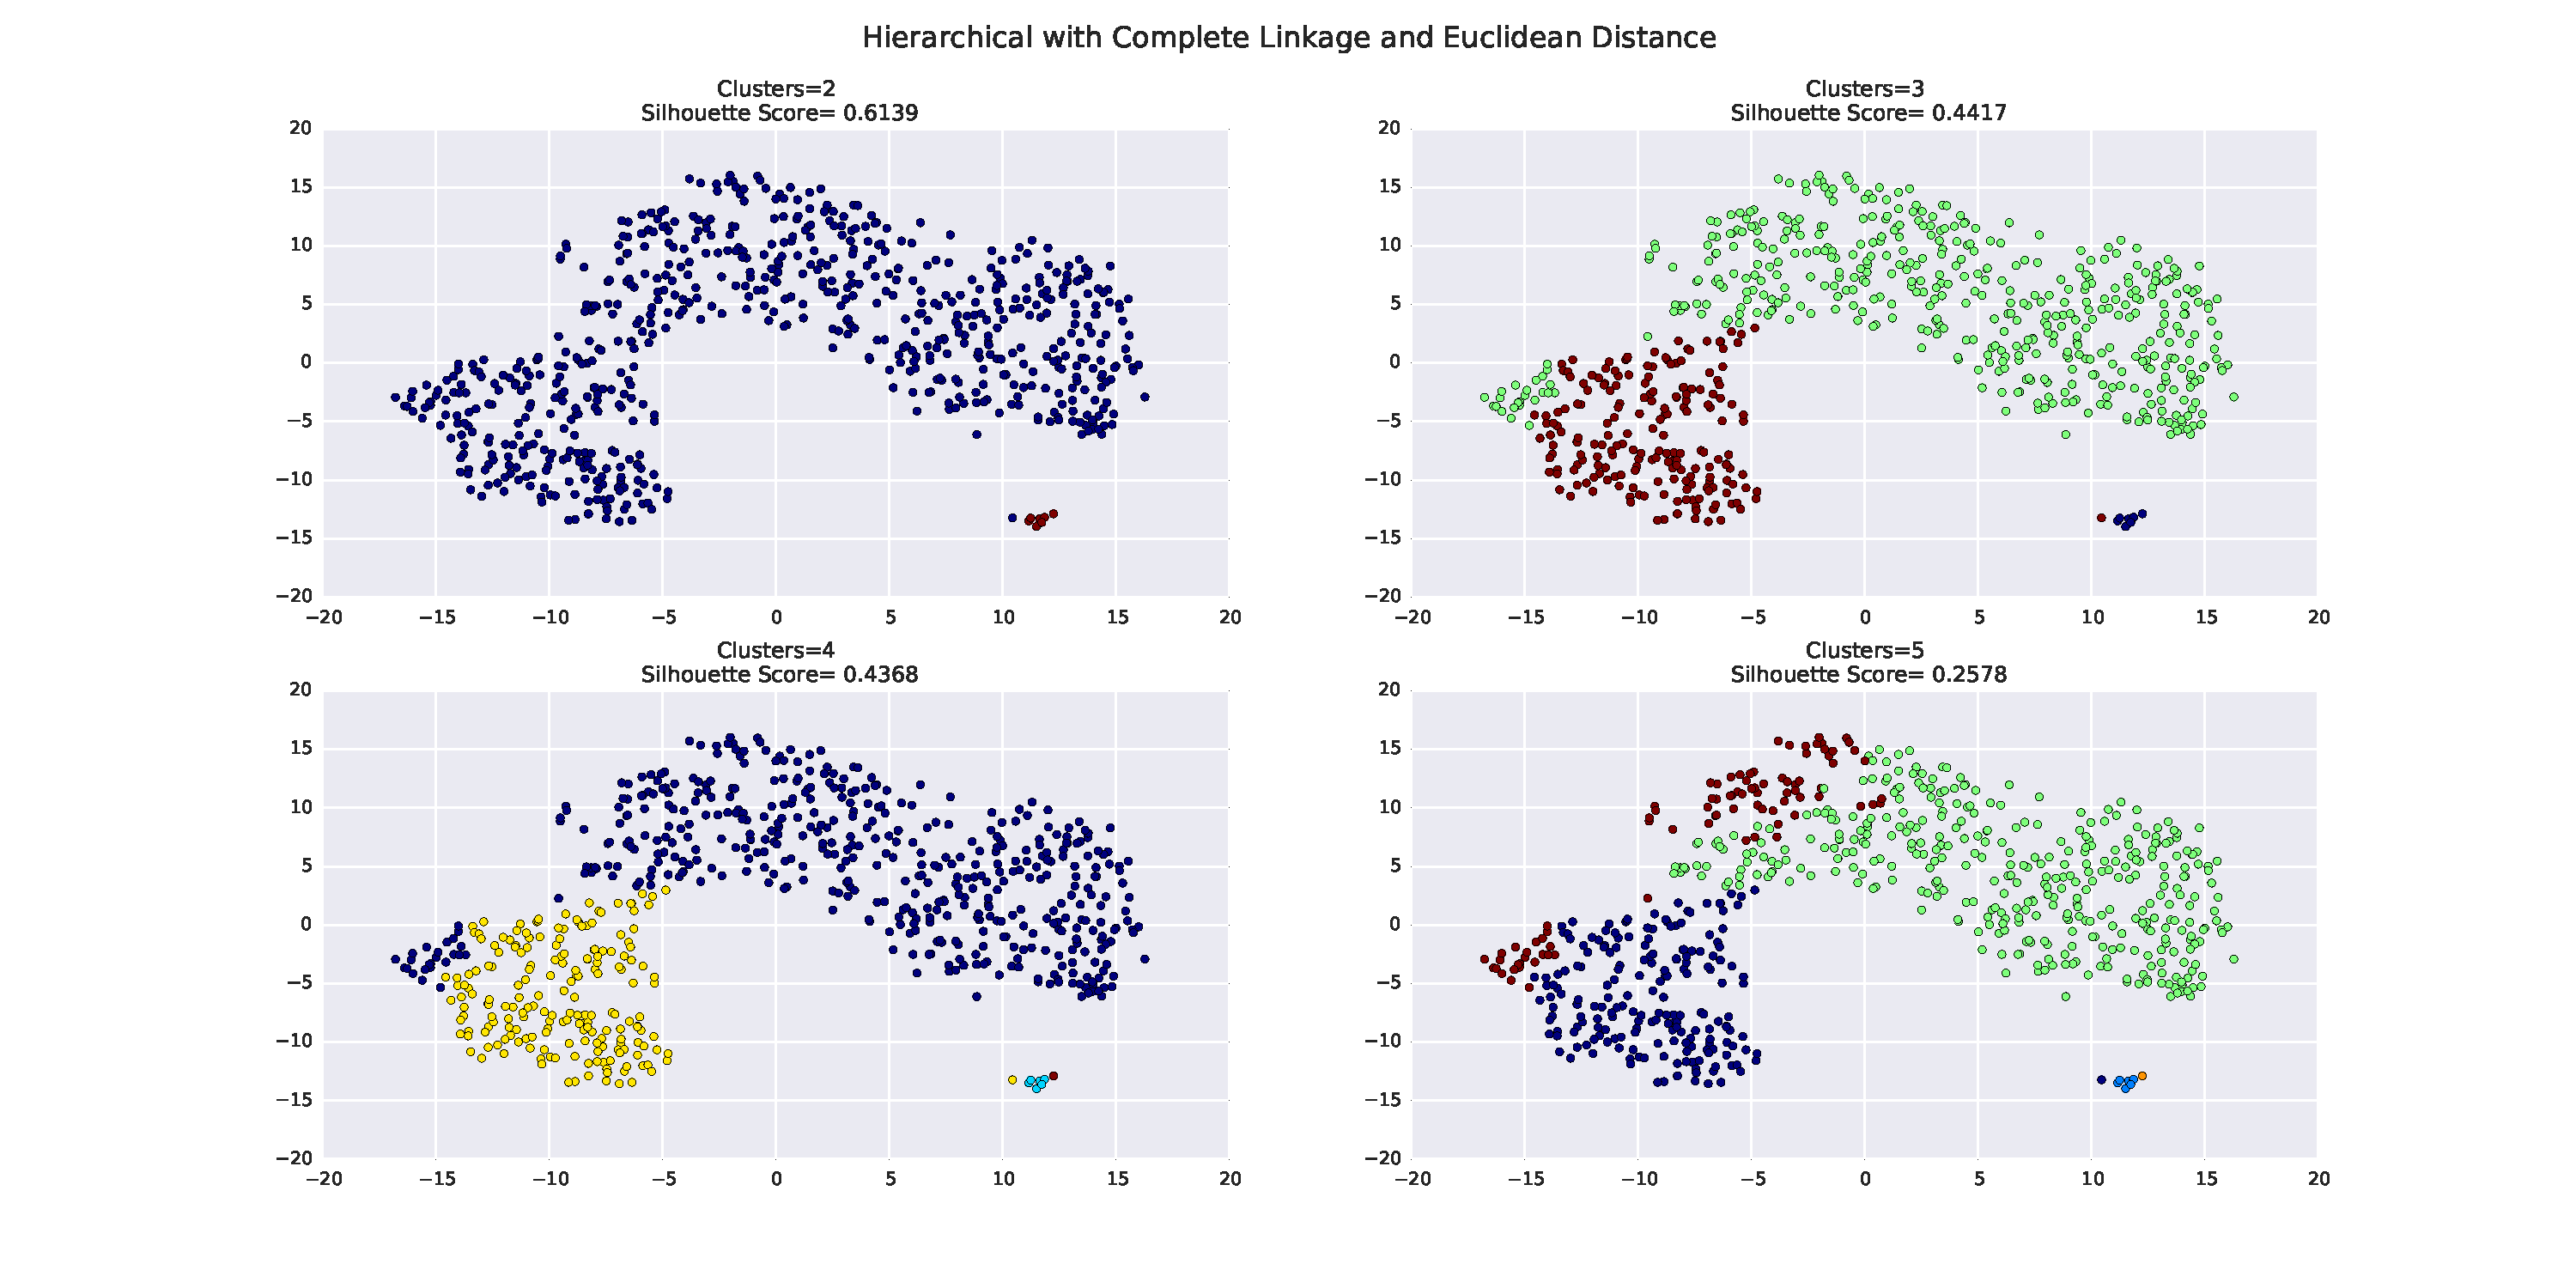
\includegraphics[width=1\textwidth]{../Code/Plots/complete_link}
  \end{center}
  \vspace{-.2cm}
  \caption{Four best Single Linkage models as we vary $1 \leq k \leq 40$.}
  \label{fig:complete_link}
  \vspace{-.1cm}
\end{figure}


\begin{figure}[htp!]
  \begin{center}
  	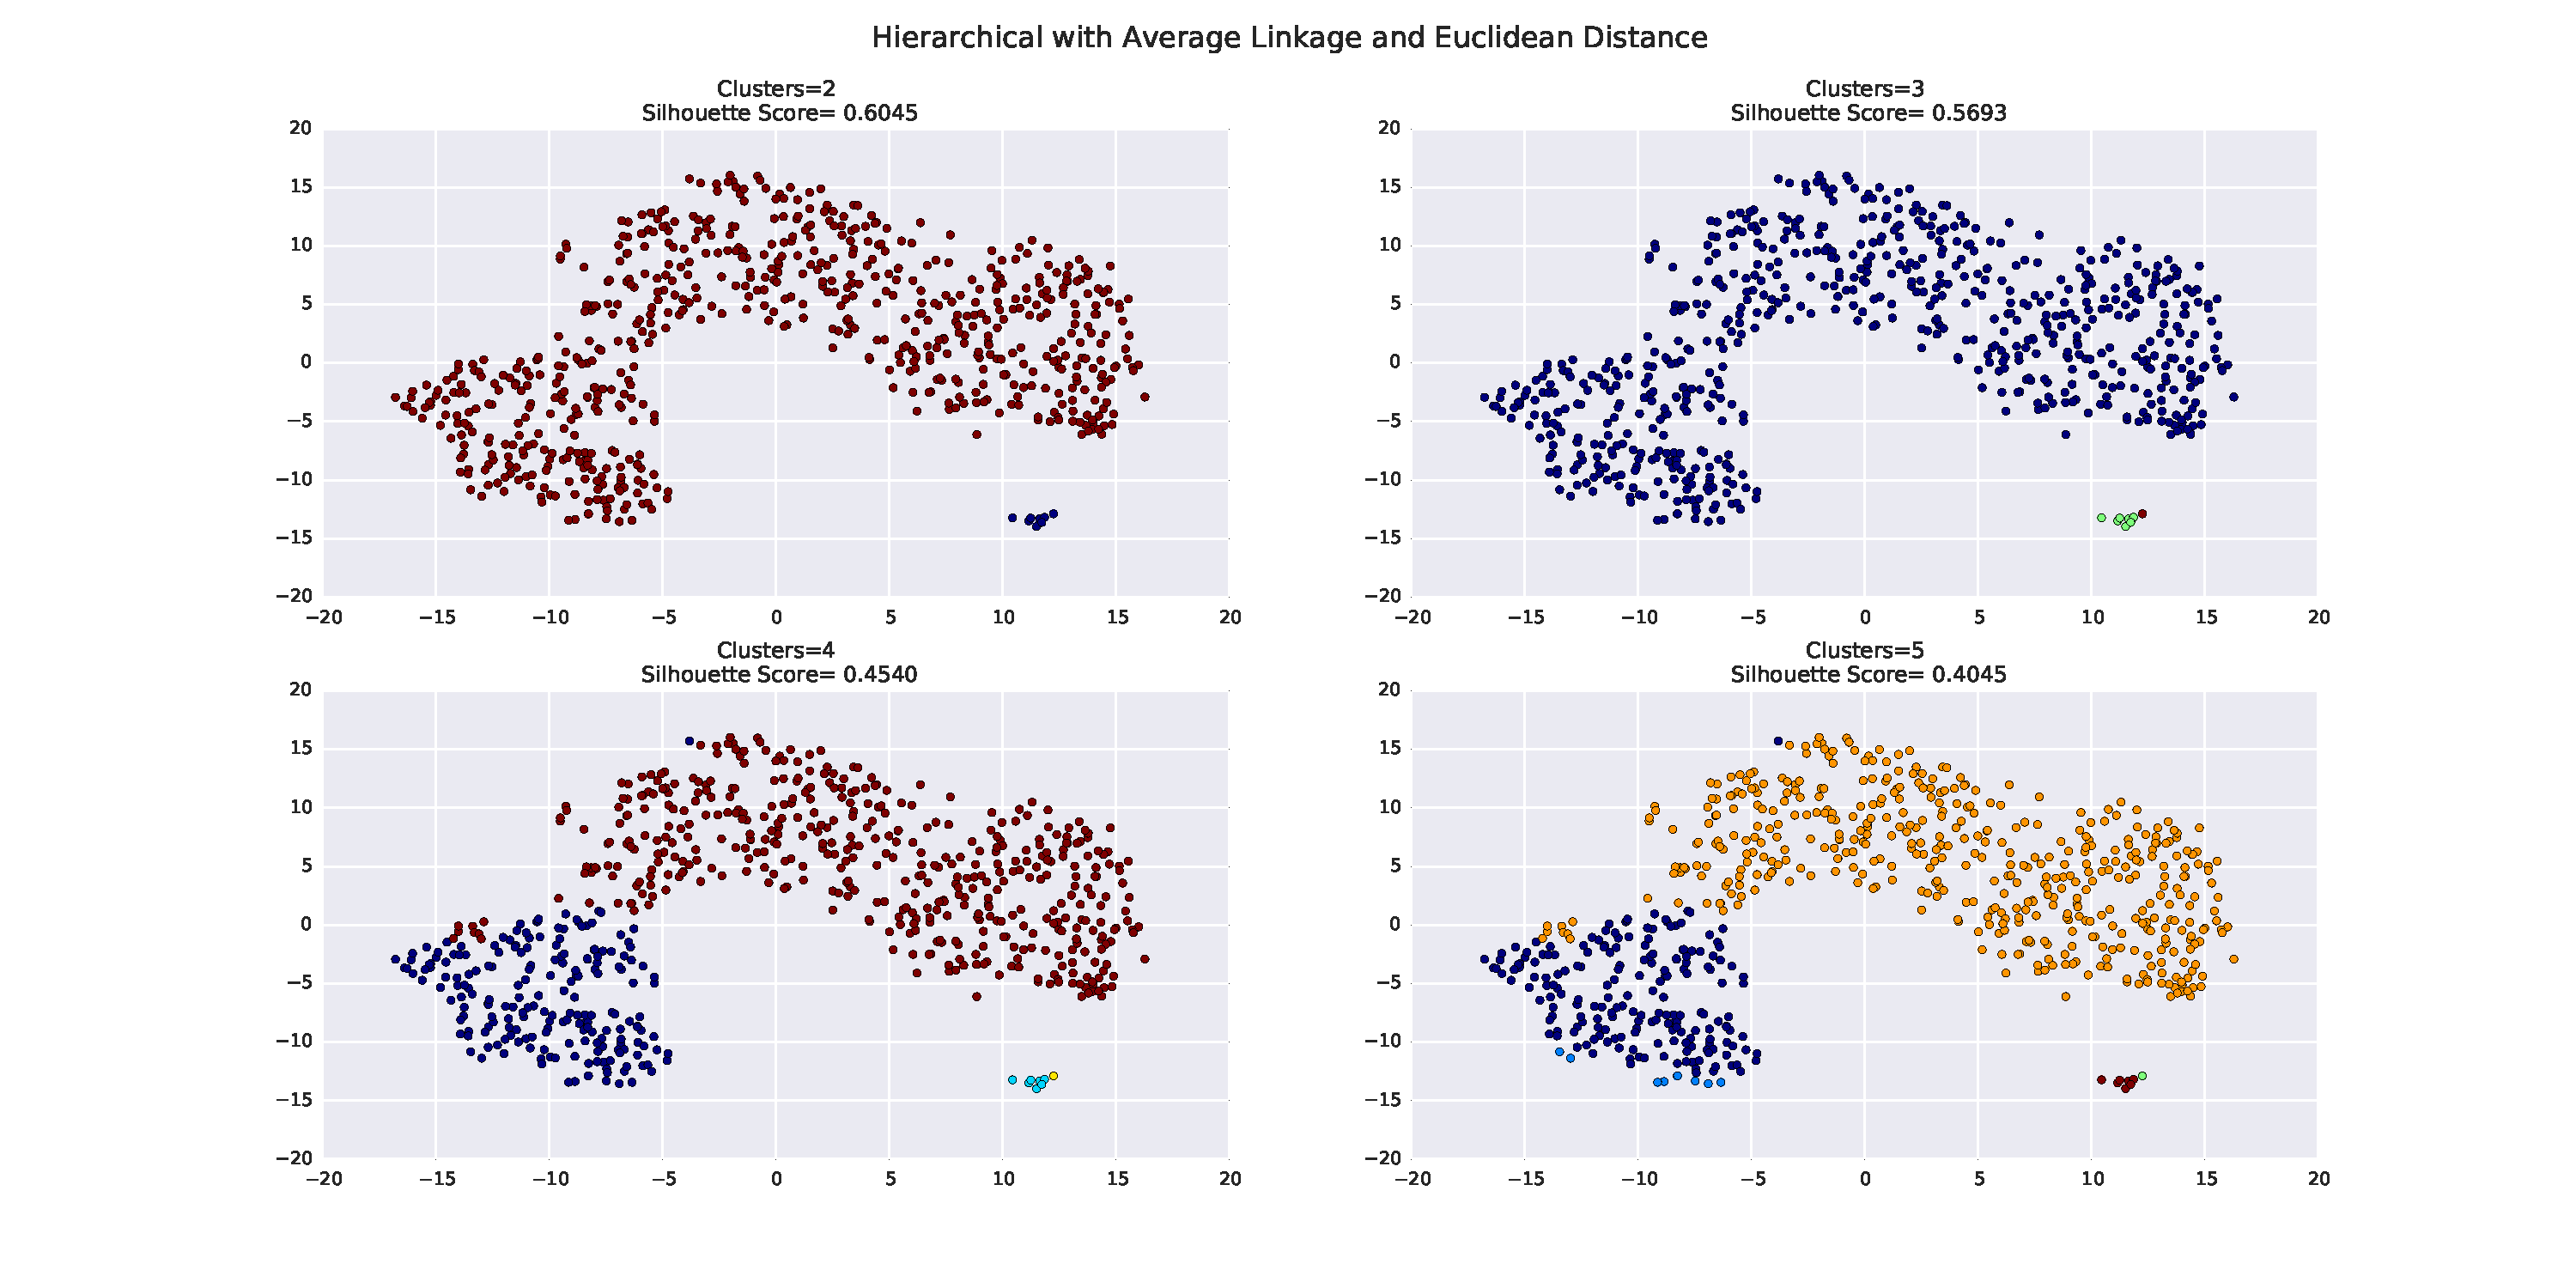
\includegraphics[width=1\textwidth]{../Code/Plots/average_link}
  \end{center}
  \vspace{-.2cm}
  \caption{Four best Single Linkage models as we vary $1 \leq k \leq 40$.}
  \label{fig:average_link}
  \vspace{-.1cm}
\end{figure}

As we see from Figures \ref{fig:single_link}, \ref{fig:complete_link}, \ref{fig:average_link}, single linkage performs the worse over the three hierarchical clustering methods. Complete linkage performs marginally better than average linkage, but again we see that the number of clusters that achieve the highest silhouette score is $k=2$. \\

Also, in Figure \ref{fig:dendro} we see the that if we let the euclidean distance be greater than $200$ we get two clear clusters.

\begin{figure}[htp!]
  \begin{center}
  	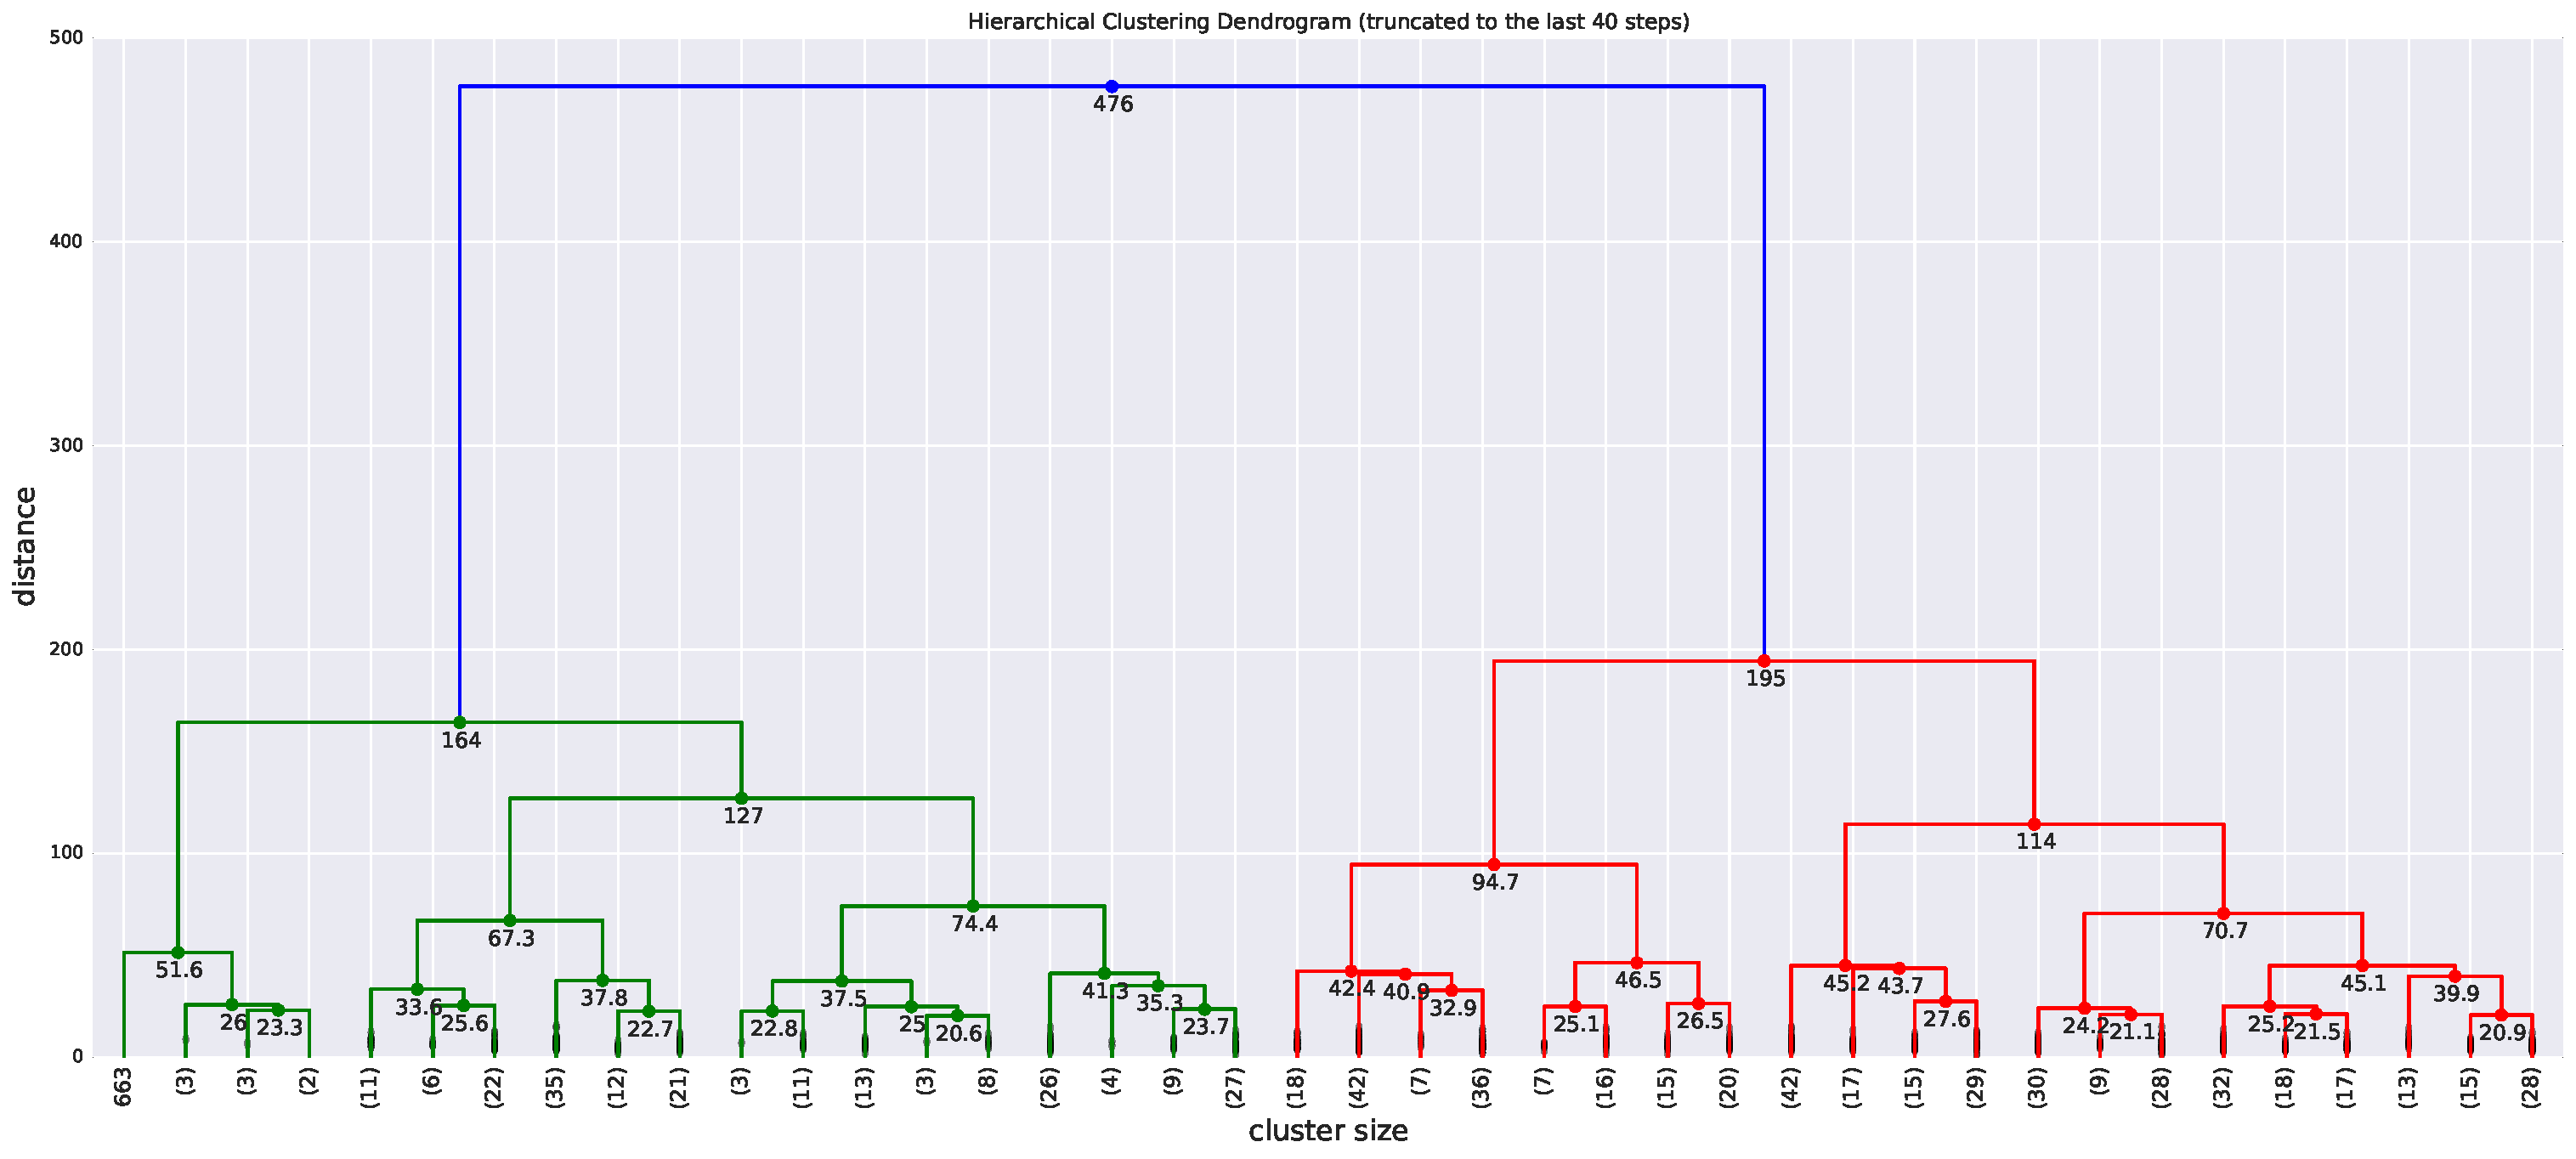
\includegraphics[width=1\textwidth]{../Code/Plots/dendro}
  \end{center}
  \vspace{-.2cm}
  \caption{Dendrogram for Complete Linkage}
  \label{fig:dendro}
  \vspace{-.1cm}
\end{figure}

\item The next clustering method that we explore, is \emph{DB-Scan}. In contrast to the previously seen clustering algorithms, in this case we do not need to supply the number of clusters, as the algorithm finds the number of clusters based on $\epsilon$ and $MinPoints$. Heuristically, we found that letting $MinPoints > 5$ always resulted in the same clustering where only one cluster was present. Therefore, we vary $1 \leq MinPoints \leq 5$ and we let $\epsilon=0.2+ 0.1t$ for $t=0, 1, \dots ,34$. As we varied $MinPoints$ between $1$ and $5$ we observed no significant changes in the value of the silhouette score. Nevertheless, the value of $\epsilon$ played a crucial role in getting a good clustering model. In fact, by looking at Figure \ref{fig:best_dbscan} we see that for $\epsilon = 2$ we get two clusters and a very high silhouette score, whereas for $\epsilon = 5$ the silhouette score is negative.
\begin{figure}[htp!]
  \begin{center}
  	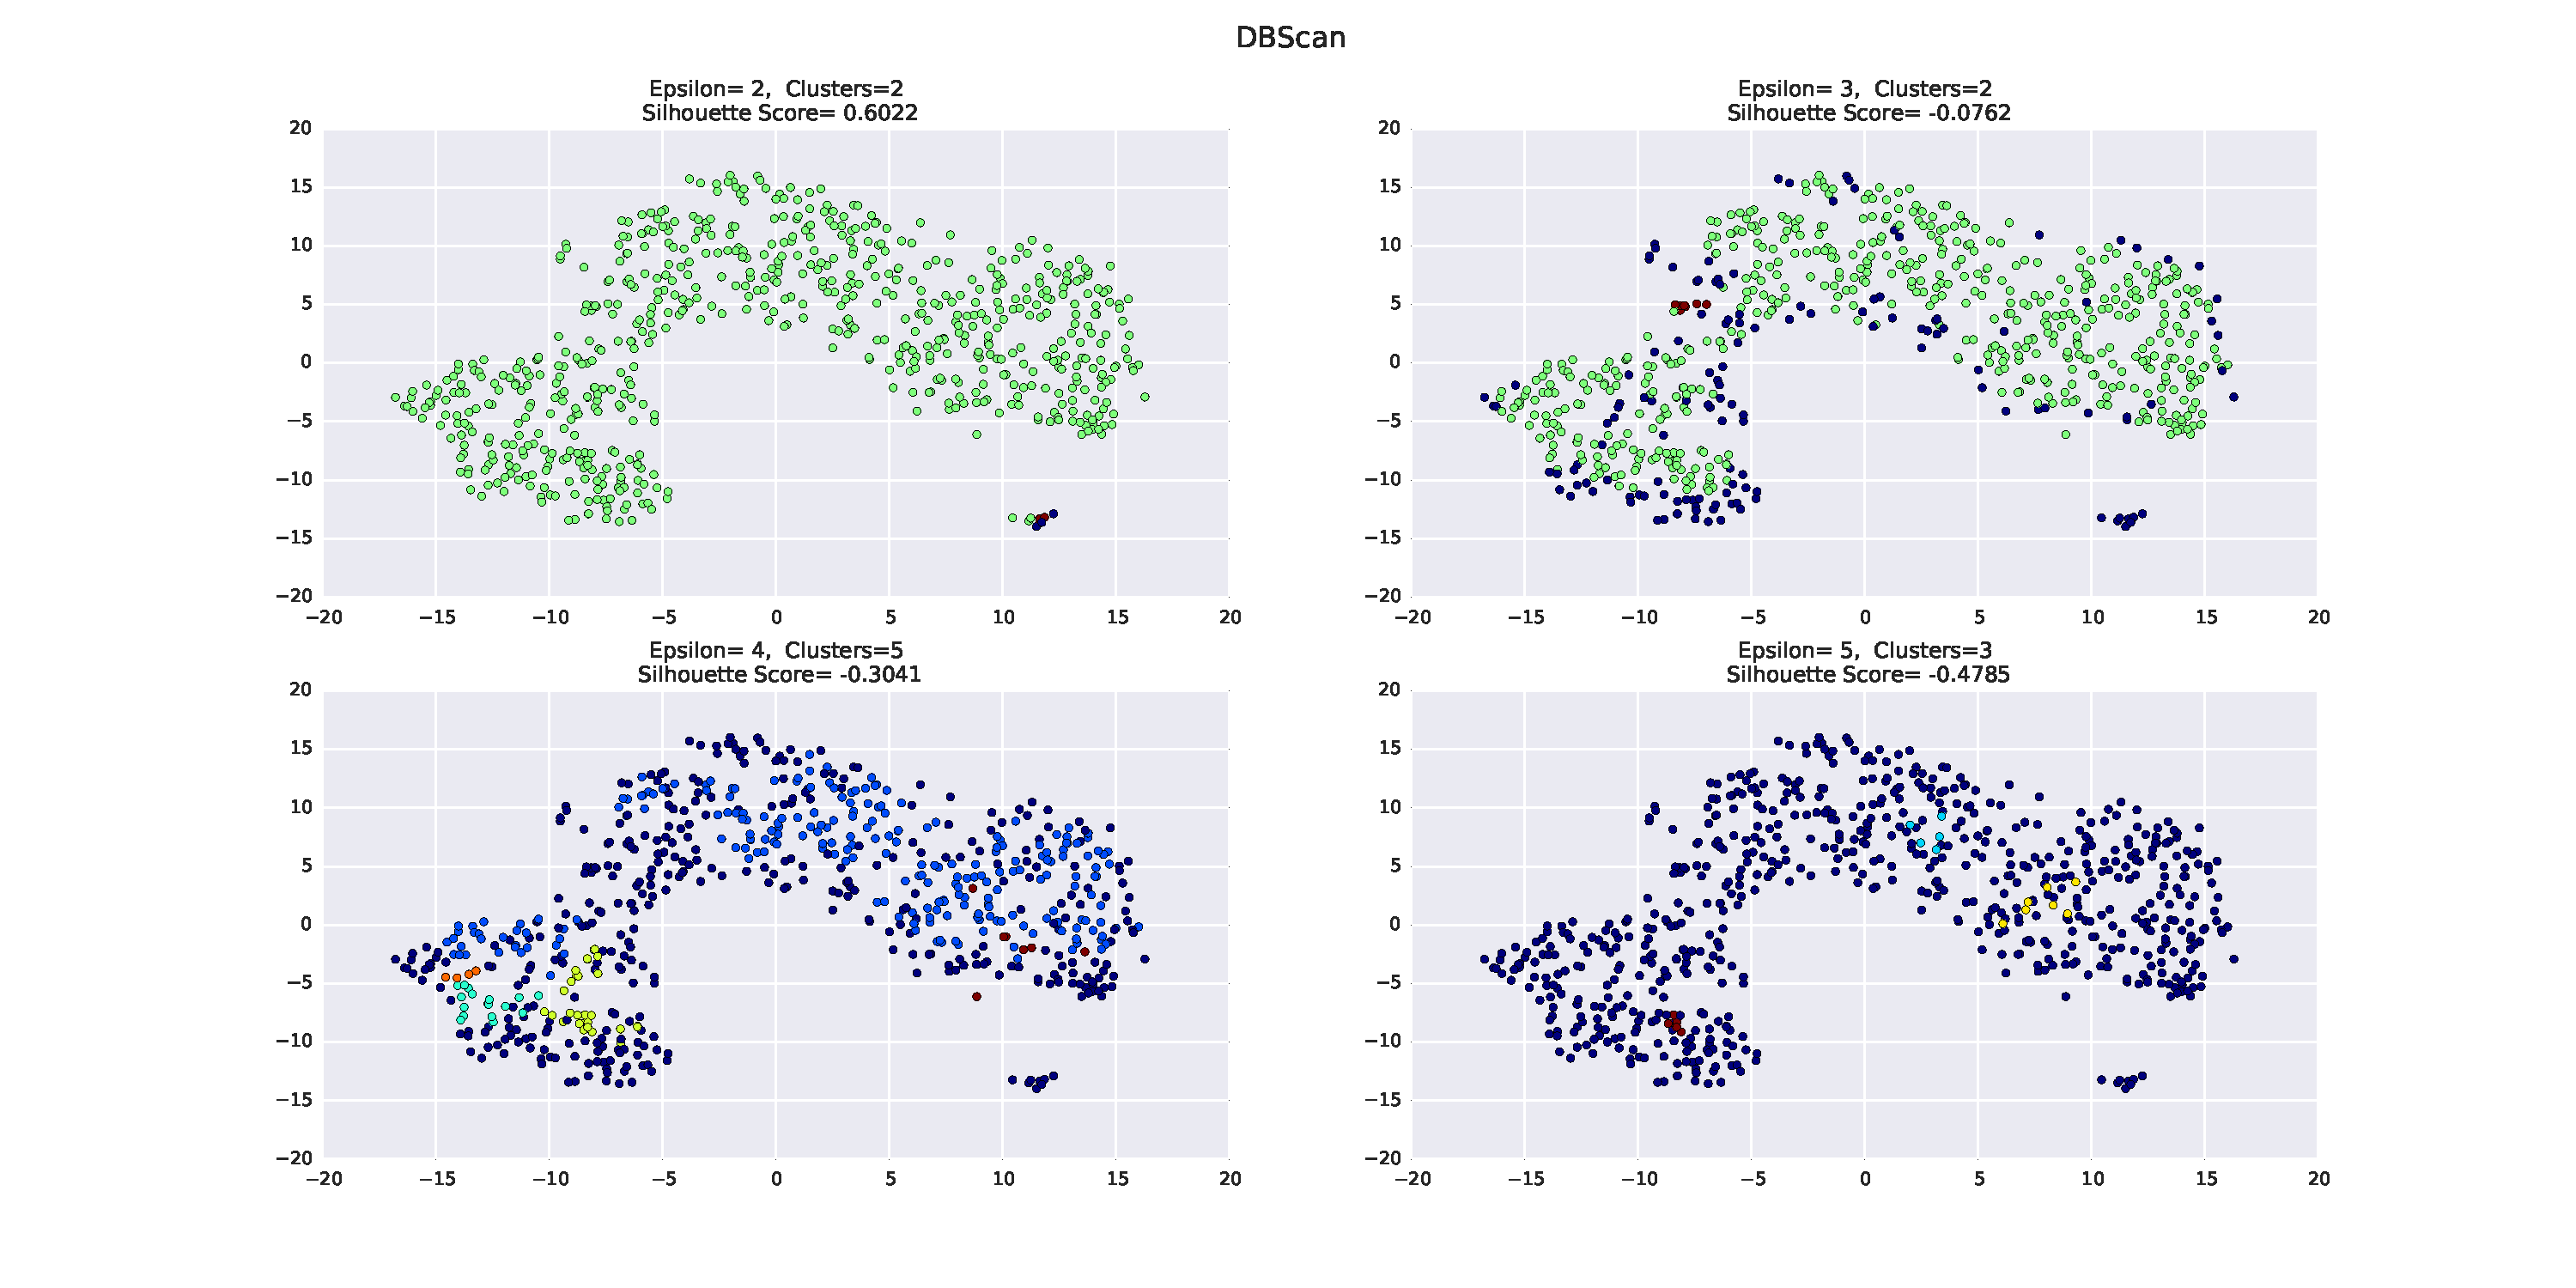
\includegraphics[width=1\textwidth]{../Code/Plots/best_dbscan_minpoints_5}
  \end{center}
  \vspace{-.2cm}
  \caption{Four best Single Linkage models as we vary $1 \leq k \leq 40$ and fix $MinPoints=5$.}
  \label{fig:best_dbscan}
  \vspace{-.1cm}
\end{figure}


\item Finally, we try the \emph{Expected Maximization} algorithm where we use Gaussian Priors. We see that this model performs very poorly compared to other clustering techniques (Fig. \ref{fig:best_gaussian}). According to this clustering model, the number of clusters that achieve the highest silhouette score ($0.1216$) is $29$, which is very different than the number of clusters suggested by our previous analysis. 

\begin{figure}[H]
  \begin{center}
  	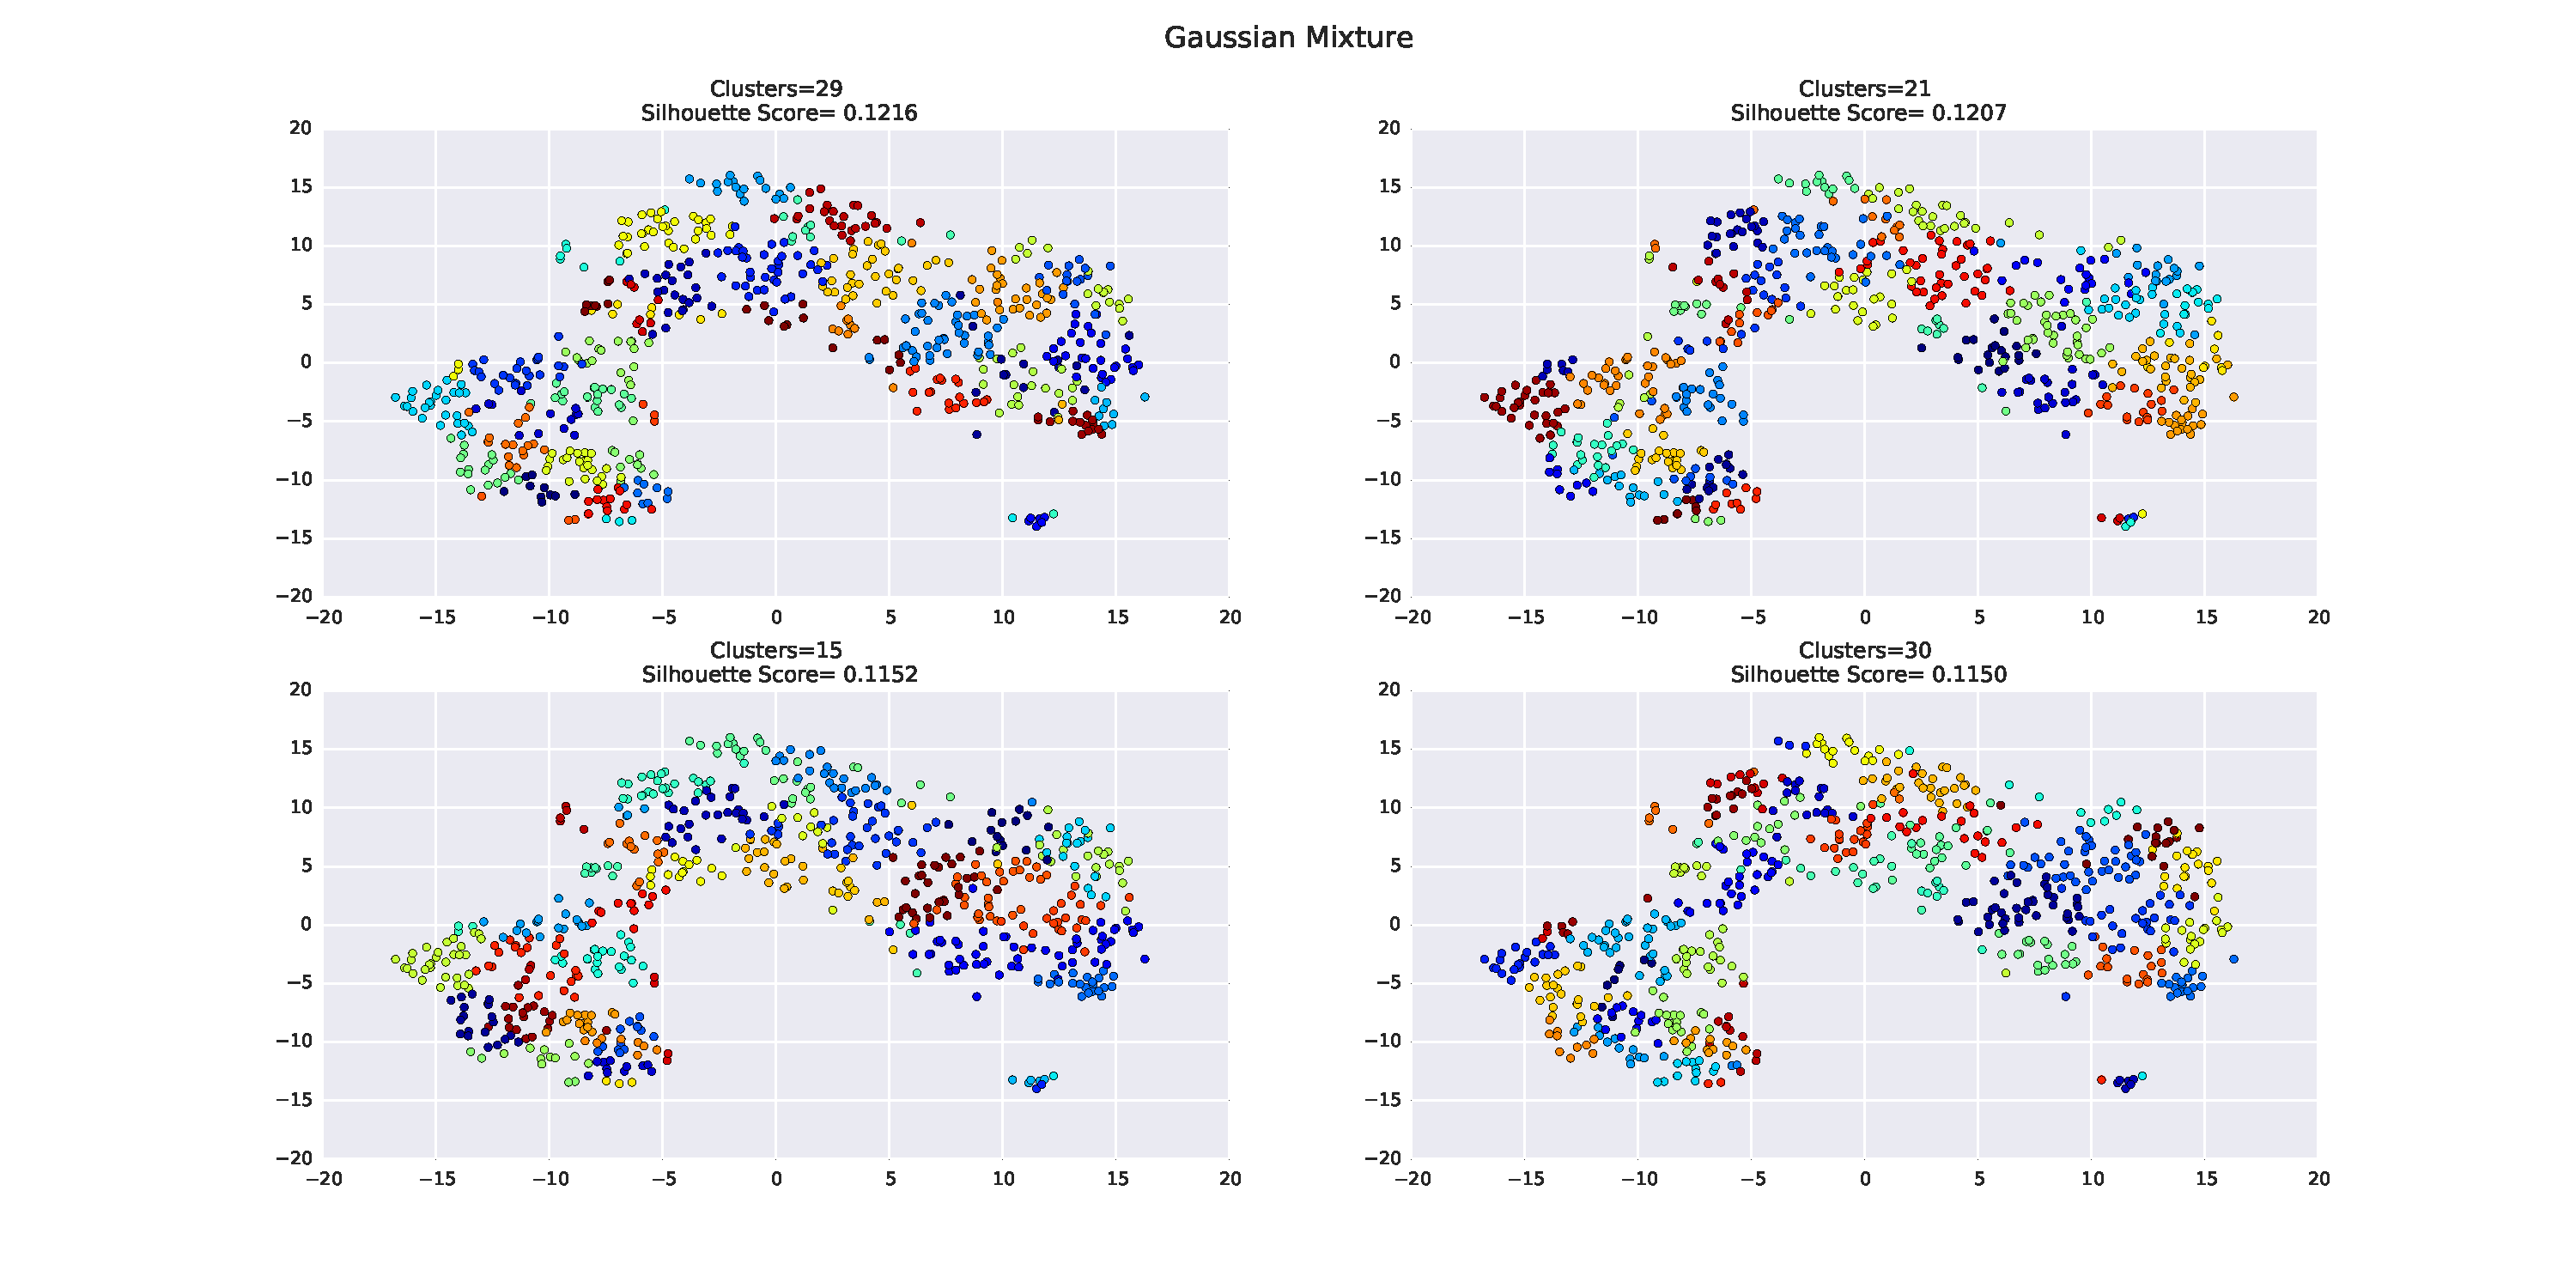
\includegraphics[width=1\textwidth]{../Code/Plots/best_gaussian}
  \end{center}
  \vspace{-.2cm}
  \caption{Four best Single Linkage models as we vary $1 \leq k \leq 40$ and fix $MinPoints=5$.}
  \label{fig:best_gaussian}
  \vspace{-.1cm}
\end{figure}


\end{enumerate}

$\implies$ Given the above analysis, we could say that one of the best clustering methods that achieves the highest silhouette score is \textbf{Agglomerative Hierarchical Clustering with Complete Linkage and number of clusters equal to two.} This method achieves a silhouette score of $0.61$, nevertheless, DB-Scan also performs very similarly achieving a silhouette score of $0.60$ for $\epsilon =2$ and total number of clusters equal to two.

\item By doing a first analysis of the data, we see that many different algorithms suggest that the most likely number of clusters is two. Investigating further, we see that in the first cluster belong only $8$ people, whereas, is in the second cluster belong around $1000$ people.\\

 By looking into the smaller of the two clusters, we see that the attributes with $0$ variance are:  \texttt{Education\_college/bachelor degree}, \texttt{Education\_currently a primary school pupil}, \texttt{Education\_primary school }, \texttt{Only child\_no}. This means that \textbf{all} people belonging in this cluster are currently attending \emph{primary} school and are not \emph{only children}. As far as other attributes are concerned, we see that in this cluster all people like \emph{Thriller} and \emph{Western} films and are \emph{left handed}, since these are the attributes with the least variance ($\sigma^{2}= 0.28, 0.68, 0.23$, respectively). \\

In the second cluster, we see that the vast majority of people really \emph{likes movies} ($\sigma^{2}=0.40$) such as \emph{comedies} ($\sigma^{2}=0.50$). Also, most people are \emph{right handed} ($\sigma^{2}=0.08$), and currently do not go to \emph{ primary school } ($\sigma^{2}=0.002$).


\item Some of the characteristics drawn from our clustering are not significant since they follow normal trends. For example most people in the country have attended primary school and are right handed. \textbf{Nevertheless}, our clustering has highlighted certain character traits that could be used in order to perform direct marketing and advertisement. For example, in the smaller cluster we see that most people are left handed, have siblings and also like Thrillers and Animated films. Similarly, it seems that right handed people opt for \emph{Comedies}. Even though many exceptions exists, and this is not an infallible trend, it gives us a vague first idea about how we could approach potential costumers. We know that within the student body, there exist two ``groups'' namely, one that mostly likes \emph{Comedies} and another one that mostly likes \emph{Thrillers and Animated films}.
\end{enumerate}


\textbf{Extra Credit:}

An alternative distance metric that we could use in order to perform clustering and measure the silhouette score is the \emph{chebysev} distance. By definition:
\[ D_{CHEB}(\vec{d_{1}},\vec{d_{2}})=  \max \left| \vec{ d_{1}}(i)-\vec{d_{2}}(i) \right| \]

This is a metric considers only one component in calculating the distance, hence we would expect to give us different results. \\

In order to see the effect of the distance metric in the silhouette score we first need to rigorously define it.  In order to compute this score, we first need to define quantities $a_i,b_i$ corresponding at point $i$ of our dataset. More precisely, let the set $\mathcal{D}$ represent the set of all data points and let $C_1 \dots C_k$ be the sequence of clusters, with $|C_j|$ being the total number of points in $C_j, 1\leq j \leq k$. Then, for a point $i \in \mathcal{D}$, let $i \in C_j$. We define: 

\[ a_i= \frac{1}{|C_j|} \sum_{e \in C_j} D(i,e)  \],
where $D(x,y)$ is an arbitrary distance function with $D(x,x)=0$ (in our case the chebysev distance). Intuitively, $a_i$ is the average distance of $i$ to all other points contained in the same cluster $C$.

Now let:
\[ b_i= \min_{\substack{w}} \left \{ \frac{1}{|C_w|} \sum_{e \in C_w} D(i,e) \right \}_{w=1, w \neq j}^{k} \]


Finally we can compute the silhouette score as: 
\[ silhouette =\frac{1}{n} \sum_{i=1}^{n} \frac{b_i - a_i}{\max(a_i,b_i)}\]

Given the above definitions, we compute the highest silhouette score that each clustering method achieved, after varying the number of clusters from $0$ to $40$: 

\begin{table}[H]
		\caption{Reporting the Silhouette Score for all clustering models. }
		\centering
        \small
		\begin{tabular}{c c c}
		\hline\hline
		{\centering Clustering Model} & 
		{ Silhouette Score }  &
		{ Clusters }
		 \\ [0.5ex] 
		\hline
        			K-Means&    		0.50& 2  \\
			Single Linkage&	0.49& 2     \\
			Complete Linkage&	0.67 & 2     \\
			Average Linkage&	\textbf{0.66} & 2    \\
			DB-Scan ($\epsilon = 2$)&			\textbf{0.66}& 2  \\
			Gaussian Mixture &	-0.02  & 5    \\
		\hline
		\end{tabular}\\[0.5cm]
		\label{table:res_singlelink}
\end{table}


From the above table, we see that using this distance metric, the silhouette score is higher for all clustering methods (except Gaussian Mixture), but the number of predicted clusters remains $2$, as in the case of the euclidean distance. \\

A possible reason for the similarity of the performance of the clustering models when we use different distance metrics, could be attributed to the fact that the maximum distance between two points ``dominates'' the euclidean metric.



\end{homeworkProblem}
% To have just one problem per page, simply put a \clearpage after each problem
%----------------------------------------------------------------------------------------
%	PROBLEM 2
%----------------------------------------------------------------------------------------

\begin{homeworkProblem}[Problem \arabic{homeworkProblemCounter}: Association Analysis]
Using the same dataset as in Problem 1, answer the following questions:
\begin{enumerate}
\item Experiment with different values for support and confidence. How do the discovered patterns change? What threshold do you recommend using for support and confidence?
\item  Identify 2-5 interesting rules generated using your selected support and confidence threshold. What is the interpretation of the rule? What is underlying rationale or reason for the rule, e.g. the diapers $\rightarrow$ beer rule was because young fathers were sent to the store to buy diapers.
\item  What are some of the potential applications of the generated rules? For example, how could the rules be used for marketing products to students?
\end{enumerate}
	
\noindent\rule{16cm}{0.9pt}
		
\large{\textbf{\underline{Answer:}}}


\begin{enumerate}


\item Based on the current code framework, the association rule formulation relies on the support and confidence measures to eliminate uninteresting patterns using the \emph{Apriori} algorithm. This method has two drawbacks, namely:
\begin{itemize} 
\item It is often the case that many potentially interesting patterns involving low support items might be eliminated by the support threshold. 
\item The drawback of confidence is more subtle. Assume for example we have an association rule \texttt{\{X\}}$\rightarrow$\texttt{\{Y\}} with very high confidence, $0.80$. The problem is that the confidence measure does not take into consideration the support of the itemset \texttt{\{Y\}}. Therefore, we could construct an example where $P(\texttt{\{Y\}}) \leq P(\texttt{\{Y\}}|\texttt{\{X\}})$, while, the confidence of the rule to be high! Thus, we would consider this to be a good rule, nevertheless, knowing that \texttt{\{X\}} occurs, actually decreases the probability of \texttt{\{Y\}} occurring.
\end{itemize}

Many alternative methods have been proposed to solve this problem such as: \emph{Interest Factor, Correlation Analysis, IS Measure} etc. In this project we use the \emph{Intertest Factor} approach to evaluate the association rules. More precisely, we evaluate the \emph{interestingness of a pattern}, by defining \emph{Lift}:

\[ Lift = \frac{ c(\texttt{\{X\}} \rightarrow \texttt{\{Y\}})} {s(\texttt{\{Y\}})} = \frac{ \sigma (\texttt{\{X\}},\texttt{\{Y\}}) } {\sigma(\texttt{\{X\}}) \sigma(\texttt{\{Y\}})} \]
, which addresses the previously discussed problem by taking into consideration the support of \texttt{\{Y\}}. From this formulation it is clear that a $Lift$ value equal to $1$ implies the statistical independence of \texttt{\{X\}}, \texttt{\{Y\}}. Therefore, we should choose rules with $Lift \gg 1$. \\

For example if we, naively, attempt to find rules that have both high support and confidence ($s=0.7, c=0.8$) we get: \\
\texttt{right handed} $\rightarrow$ \texttt{Music=5}, which has $Lift \approx 1$, therefore it is a bad rule. \\

Also, setting both support and confidence to low values ($s=0.1, c=0.2$) produces very obvious  results with high $Lift$ values:\\
 \texttt{right handed,Only.child=yes, city} $\rightarrow$ \texttt{Number.of.siblings=0}.
 The above pattern is achieves a $Lift$ score of $5$, nevertheless, it is not informative since we already know that an only child has no siblings.\\
 
 After experimentation, the values that yield the most informative results are $\sigma \approx 0.1$ and $c \approx 0.5$.
 
 \item Some of the most interesting rules that we see are :
 
 \begin{itemize}
 \item \texttt{Biology=5} $\rightarrow$ \texttt{Chemistry=5}: This rules achieves a Lift score of $5.2$, and it implies that if a persons likes Biology then he is also very likely to like Chemistry. This is a logical rule since these two fields are closely related.
 \item \texttt{Fun.with.friends=5, Shopping.centres=5, Gender=female} $\rightarrow$ \texttt{Shopping=5}: This rules achieves a Lift score of $4.3$, and it implies that females who like shopping centers and also to have fun with friends, are also very probable to like shopping. The underlying rational behind this rule is, that if a female likes spending time in shopping centers, then she is also likely to start shopping.
 \item \texttt{Internet=5, Gender=male, city} $\rightarrow$ \texttt{PC=5}: Achieving a Lift score of $4.1$, this rule implies that a male who likes internet and lives in the city, is also very likely to like PCs. This is also a logical rule, since the internet and PCs have an immediate connection.
 
 
 \end{itemize}
 
 \item All of the aforementioned rules, could be used by companies for direct advertising. For example, if a company like Amazon observes that a student has bought a Biology book then it can suggest a Chemistry book to the student as well. Also, if a female likes visiting shopping centers and being around friends, then a company could offer free shopping coupons to that student in order to make some product more enticing. Finally, companies in big cities, such as Xfinity, that know that a particular male consumer likes browsing on the internet, can offer to this student specialized PC offers in order to attract him. 
 
 
 \end{enumerate}
       
 \end{homeworkProblem}





\end{document}
